\subsection{完备群}

定义 2 拓扑群称为完备的，如果它的左一致结构与右一致结构都是完备空间的结构。

由第 1 目命题 2，为使一个群是完备的，只需它的两个一致结构之一是完备空间的结构。G 完备当且仅当它的伴随 Hausdorff 群（§ 2 第 6 目）完备。

完备群的每个闭子群是完备的（第二章 § 3 第 4 目命题 8）。完备群的每个积是完备的（第二章 § 3 第 5 目命题 10）。

\pandocbounded{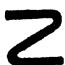
\includegraphics[keepaspectratio]{images/part002_8d186292.jpg}}

另一方面，若 G 是一个完备群且 H 是 G 的一个闭正规子群，则商群 G/H 未必完备（但参看第九章 § 3 第 1 目命题 4）。

命题 4 若在拓扑群 G 中存在 e 的一个邻域 V，它关于右一致结构或左一致结构之一是完备的，则 G 是完备的。

例如设 V 关于右一致结构是完备的，并设 F 是 \(G_{d}\) 上的一个 Cauchy 滤子；则 F 含有一个 \(V_{d}\)-小集 M，且若 \(x_{1} \in M\)，我们因而有 \(M \subset Vx_{1}\)。于是 F 在完备子空间 \(Vx_{1}\)（\(G_{d}\) 的）上的迹是一个 Cauchy 滤子，它收敛于一点 \(x_{0}\)；由于 \(x_{0}\) 是 F 的聚点，它是 F 的极限（第二章 § 3 第 2 目命题 5 推论 2）。

推论 1 局部紧群是完备的。

因为每个紧空间关于它的唯一的一致结构是完备的（第二章 § 4 第 1 目定理 1）。

推论 2 Hausdorff 拓扑群 G 的每个局部紧子群在 G 中是闭的。

因为 Hausdorff 一致空间的每个完备子空间是闭的（第二章 § 3 第 4 目命题 8）。

命题 5 设 \(G_{1}\) 是一个拓扑群，\(G_{2}\) 是一个完备的 Hausdorff 拓扑群，\(H_{1}\)（相应地 \(H_{2}\)）是 \(G_{1}\)（相应地 \(G_{2}\)）的一个稠密子群。则 \(H_{1}\) 到 \(H_{2}\) 中的每个连续同态 u 可以唯一地延拓为一个连续同态 \(\overline{u}\)（\(G_{1}\) 到 \(G_{2}\) 中的）。此外，若 \(G_{1}\) 是 Hausdorff 的且完备的，且 u 是 \(H_{1}\) 到 \(H_{2}\) 上的一个同构，则 \(\overline{u}\) 是 \(G_{1}\) 到 \(G_{2}\) 上的一个同构。

\(\overline{u}\) 关于 \(\mathbf{H}_1\) 与 \(\mathbf{H}_2\) 的右一致结构是一致连续的（第 1 目命题 3），因而容许唯一的延拓：映射 \(\overline{u}\)（\(\mathbf{G}_1\) 到 \(\mathbf{G}_2\) 中的），它关于这些群的右一致结构是一致连续的（第二章 § 3 第 6 目定理 2）。此外，依据恒等延拓原理（第一章 § 8 第 1 目命题 2 推论 1），\(\overline{u}\) 是 \(\mathbf{G}_1\) 到 \(\mathbf{G}_2\) 中的一个同态，由此得到命题的第一个断言。为证明第二个断言，只需考虑同构 \(v\)（\(\mathbf{H}_2\) 到 \(\mathbf{H}_1\) 上的，它是 \(u\) 的逆），以及它的延拓 \(\overline{v}\)（到 \(\mathbf{G}_2\) 到 \(\mathbf{G}_1\) 中的一个连续同态上的）；由于延拓的唯一性，\(\overline{v} \circ \overline{u}\) 与 \(\overline{u} \circ \overline{v}\) 分别是 \(\mathbf{G}_1\) 与 \(\mathbf{G}_2\) 的恒等映射，因而（《集合论》，R，§ 2，第 12 目）\(\overline{u}\) 是双射。

\pandocbounded{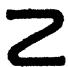
\includegraphics[keepaspectratio]{images/part002_2e6b534c.jpg}}

注。若连续同态 \(u\) 是双射，一般不能推出 \(\overline{u}\) 是单射或满射（参看习题 12）；但参看第 5 目命题 9。

